\documentclass[final]{beamer}

\usepackage{tikz}
\usetikzlibrary{arrows,shapes}
\usepackage{graphics}
\mode<presentation>{\usetheme{UNSWNICTA}}
\usepackage[english]{babel}
\usepackage[latin1]{inputenc}
\usepackage{amsmath,amsthm, amssymb, latexsym}
\boldmath
\usepackage[orientation=portrait,size=a0,scale=1.4,debug]{beamerposter}

%%%%%%%%%%%%%%%%%%%%%%%%%%%%%%%%%%%%%%%%%%%%%%%%%%%%%%%%%%%%%%%%%%%%%%%%%%%%%%%%%%%%%%

\title{\huge CNF Encodings for the Car Sequencing Problem}
\author{Valentin Mayer-Eichberger and Toby Walsh}
\institute[UNSW]{NICTA and University of New South Wales, Australia}

%%%%%%%%%%%%%%%%%%%%%%%%%%%%%%%%%%%%%%%%%%%%%%%%%%%%%%%%%%%%%%%%%%%%%%%%%%%%%%%%%%%%%%

\newlength{\columnheight}
\setlength{\columnheight}{105cm}

%%%%%%%%%%%%%%%%%%%%%%%%%%%%%%%%%%%%%%%%%%%%%%%%%%%%%%%%%%%%%%%%%%%%%%%%%%%%%%%%%%%%%%
\begin{document}
\begin{frame}
  \begin{columns}
    % ---------------------------------------------------------%
    % Set up a column 
    \begin{column}{.49\textwidth}
      \begin{beamercolorbox}[center,wd=\textwidth]{postercolumn}
        \begin{minipage}[T]{.95\textwidth}  % tweaks the width, makes a new \textwidth
          \parbox[t][\columnheight]{\textwidth}{ % must be some better way to set the the height, width and textwidth simultaneously
            % Since all columns are the same length, it is all nice and tidy.  You have to get the height empirically
            % ---------------------------------------------------------%
            % fill each column with content            
            \begin{block}{Introduction}
              \begin{columns}
                \begin{column}{.55\textwidth}
                    \begin{itemize}
                        \item Cars require different options (air-conditioning, sun-roof, etc.)
                        \item Is there a production sequence for cars on the assembly line satisfying the sliding capacity constraints?
                        \item CSPLib Benchmark Nr. 1
                    \end{itemize}
                \end{column}
                \begin{column}{.44\textwidth}
                  \centering
                    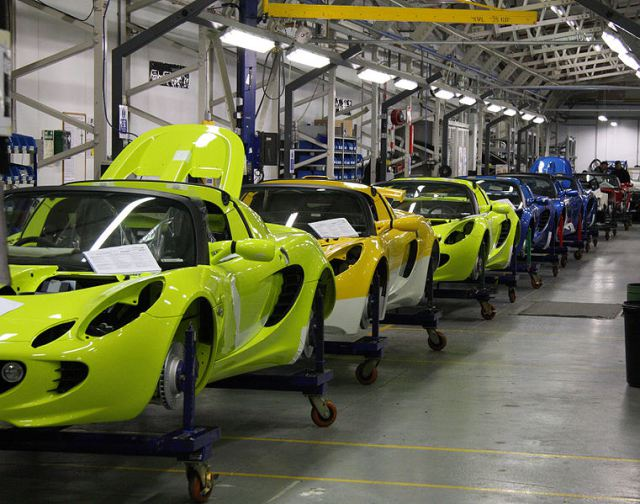
\includegraphics[width=0.80\linewidth]{figures/cars}
                \end{column}
            \end{columns}
            \end{block}
            \vfill
            \begin{block}{Example}

                \begin{itemize}
                \itemsep1pt\parskip0pt\parsep0pt
                \item
                  Classes $C = \{1,2,3\}$ with demand $d_1=3, d_2=2,d_ 3=2$
                \item
                  Options $O = \{a,b\}$ with capacity constraints $1/2$ and $1/5$
                \item
                    Class 1: $\emptyset$, Class 2: $\{a\}$, Class 3: $\{a,b\}$
                \end{itemize}
                
                \vspace{0.5cm}
                
                \begin{center}
                \begin{tabular}{c|cccccccc}
                Sequence of cars  & 3 & 1 & 2 & 1 & 2 & 1 & 3 \\
                \hline
                Option $a$ & 1 & - & 1 & - & 1 & - & 1 \\
                Option $b$ & 1 & - & - & - & - & - & 1 \\
                \end{tabular}
                \end{center}

              \vskip-1ex
            \end{block}
            \vfill
            \begin{block}{PB Model}
                \begin{itemize}
                \itemsep1pt\parskip0pt\parsep0pt
                \item
                  Boolean variable $c^k_i$: car $k\in C$ is at position $i$
                \item
                  Boolean variable $o^l_i$: option $l\in O$ is at position $i$
                \item
                  Demand constraints: $\forall k \in C$ \[\sum^n_{i=1} c^k_i = d_k\]\\
                \item
                  Capacity constraints: $\forall l \in O$ with ratio $u_l/q_l$
                  \[\bigwedge_{i=0}^{n-q_l}(\sum_{j=1}^{q_l} o^l_{i+j} \leq u_l )\]
                \end{itemize}
                
                And in all positions $i \in \{1\ldots n\}$ of the sequence it must hold:
                
                \begin{itemize}
                    \item Link between classes and options: for each $k\in C$ and 
                        \begin{align*}
                            \forall l \in O_k :\;\; & c^k_i - o^l_i \leq 0 \\
                            \forall l \in O \setminus O_k :\;\; &c^k_i + o^l_i \leq 1\\
                        \end{align*}
                    \item Exactly one car:  $$\sum_{k\in C} c^k_i = 1$$  
                \end{itemize}
            \end{block}
            \vfill
            \begin{block}{SAT Approach: The Ultimate Decomposition}
                \begin{itemize}
                \itemsep1pt\parskip0pt\parsep0pt
                \item
                  ONE constraint: e.g. $a \vee b \vee \neg c$.
                \item
                  ONE propagator: e.g. $a$ and $\neg a \vee b$ then propagate $b$.
                \item
                  Use SAT solver as a blackbox and inherit all good properties!
                \item
                  Central constraint: $(\sum_{i=1}^n x_{i} = d) \wedge\bigwedge_{i=0}^{n-q}(\sum_{l=1}^q x_{i+l} \leq u )$
                \item
                  Use cumulative sums:
                \end{itemize}

                    $$ s_{i,j} \iff (j \leq \sum_{l=1}^{i} x_{l}) $$
                
                

            \end{block}
            \vfill
            \begin{block}{Counter based Clause Set}%
                \begin{center}
                                          
                \begin{tikzpicture}[scale=3.0,node distance=1cm, auto,]
                \tikzstyle{myarrows}=[line width=1mm,-triangle 45,postaction={draw, line width=3mm, shorten >=4mm, -}]
                \coordinate (A) at (0.5,1.1);
                \coordinate (B) at (1.5,1.1);
                \coordinate (C) at (0.5,-0.1);
                \coordinate (D) at (1.5,-0.1);
                                   
                \draw (0, 0) rectangle (1, 1);
                \draw (1, 0) rectangle (2, 1);
                \draw[->,myarrows] (A) to [bend left] (B);
                \draw[->,myarrows] (D) to [bend left] (C);
                
                
                \node at (0.5,0.5) {$s_{i-1,j}$};
                \node at (1.5,0.5) {$s_{i,j}$};
                \node at (1,-0.5) {$\neg x_i$};
                
                \node at (8,1) {$\neg s_{i-1,j} \vee s_{i,j}$};
                \node at (8,0) {$x_{i} \vee \neg s_{i,j} \vee s_{i-1,j}$};
                
                \end{tikzpicture}
                \end{center}
                
                \vspace{1cm}
                \begin{center}
                \begin{tikzpicture}[scale=3.0,node distance=1cm, auto,]
                \tikzstyle{myarrows}=[line width=1mm,-triangle 45,postaction={draw, line width=3mm, shorten >=4mm, -}]
                
                \coordinate (A) at (0.1,1.1);
                \coordinate (B) at (0.9,1.9);
                \coordinate (C) at (1.1,0.1);
                \coordinate (D) at (1.9,0.9);
                
                \draw (0, 0) rectangle (1, 1);
                \draw (1, 1) rectangle (2, 2);
                \draw[->,myarrows] (A) to [bend left] (B);
                \draw[->,myarrows] (D) to [bend left] (C);
                
                \node at (0.7,0.5) {$s_{i-1,j-1}$};
                \node at (1.5,1.5) {$s_{i,j}$};
                \node at (0,1.8) {$x_i$};
                
                \node at (8,1.5) {$\neg x_{i} \vee \neg s_{i-1,j-1} \vee s_{i,j}$};
                \node at (8,0.5) {$\neg s_{i,j} \vee s_{i-1,j-1}$};
                \end{tikzpicture}

                \vspace{1cm}

                \begin{tikzpicture}[scale=3.0,node distance=1cm, auto,]
                \tikzstyle{myarrows}=[line width=1mm,-triangle 45,postaction={draw, line width=3mm, shorten >=4mm, -}]
                
                \coordinate (A) at (0.5,1.1);
                \coordinate (B) at (3.9,2.5);
                
                \draw (0, 0) rectangle (1, 1);
                \draw (4, 2) rectangle (5, 3);
                \draw[->,myarrows] (B) to [bend right] (A);
                
                \draw[dashed] (4.5,0.5) -- (4.5,2);
                \draw[dashed] (1.5,0.5) -- (4.5,0.5);
                
                \node at (0.7,0.5) {$s_{i-q,j-u}$};
                \node at (4.5,2.5) {$s_{i,j}$};
                
                \node at (5.1,1.5) {$u$};
                \node at (2.5,0) {$q$};
                
                \node at (8,2) {$\neg s_{i,j} \vee s_{i-q,j-u}$};
                
                \end{tikzpicture}
                \end{center}
            %   
            \end{block}
            \vfill
          }
        \end{minipage}
      \end{beamercolorbox}
    \end{column}
    % ---------------------------------------------------------%
    % end the column

    % ---------------------------------------------------------%
    % Set up a column 
    \begin{column}{.49\textwidth}
      \begin{beamercolorbox}[center,wd=\textwidth]{postercolumn}
        \begin{minipage}[T]{.95\textwidth} % tweaks the width, makes a new \textwidth
          \parbox[t][\columnheight]{\textwidth}{ % must be some better way to set the the height, width and textwidth simultaneously
            % Since all columns are the same length, it is all nice and tidy.  You have to get the height empirically
            % ---------------------------------------------------------%
            % fill each column with content
            
            \begin{block}{Example: 22 Cars, Capacity $4/8$, Demand $d=12$}

                %\begin{tikzpicture}
\node [matrix,ampersand replacement=\&,nodes={minimum size=6mm}]
%,nodes={fill=blue!20,minimum size=5mm}] 
    {
\node{13}; \& \node (x) { }; \& \node { }; \& \node { }; \& \node { }; \& \node { }; \& \node { }; \& \node { }; \& \node { }; \& \node { }; \& \node { }; \& \node { }; \& \node { }; \& \node { }; \& \node { }; \& \node { }; \& \node { }; \& \node { }; \& \node { }; \& \node { }; \& \node { }; \& \node {U}; \& \node {U}; \& \node {U}; \\
\node{12}; \& \node { }; \& \node { }; \& \node { }; \& \node { }; \& \node { }; \& \node { }; \& \node { }; \& \node { }; \& \node { }; \& \node { }; \& \node { }; \& \node { }; \& \node { }; \& \node { }; \& \node { }; \& \node { }; \& \node { }; \& \node { }; \& \node { }; \& \node {U}; \& \node {?}; \& \node {?}; \& \node {L}; \\
\node{11}; \& \node { }; \& \node { }; \& \node { }; \& \node { }; \& \node { }; \& \node { }; \& \node { }; \& \node { }; \& \node { }; \& \node { }; \& \node { }; \& \node { }; \& \node { }; \& \node { }; \& \node { }; \& \node { }; \& \node { }; \& \node { }; \& \node {U}; \& \node {?}; \& \node {?}; \& \node {L}; \& \node { }; \\
\node{10}; \& \node { }; \& \node { }; \& \node { }; \& \node { }; \& \node { }; \& \node { }; \& \node { }; \& \node { }; \& \node { }; \& \node { }; \& \node { }; \& \node { }; \& \node { }; \& \node { }; \& \node { }; \& \node { }; \& \node { }; \& \node {U}; \& \node {?}; \& \node {?}; \& \node {L}; \& \node { }; \& \node { }; \\
\node{9}; \& \node { }; \& \node { }; \& \node { }; \& \node { }; \& \node { }; \& \node { }; \& \node { }; \& \node { }; \& \node { }; \& \node { }; \& \node { }; \& \node { }; \& \node {U}; \& \node {U}; \& \node {U}; \& \node {U}; \& \node {U}; \& \node {?}; \& \node {?}; \& \node {L}; \& \node { }; \& \node { }; \& \node { }; \\
\node{8}; \& \node { }; \& \node { }; \& \node { }; \& \node { }; \& \node { }; \& \node { }; \& \node { }; \& \node { }; \& \node { }; \& \node { }; \& \node { }; \& \node {U}; \& \node {?}; \& \node {?}; \& \node {L}; \& \node {L}; \& \node {L}; \& \node {L}; \& \node {L}; \& \node { }; \& \node { }; \& \node { }; \& \node { }; \\
\node{7}; \& \node { }; \& \node { }; \& \node { }; \& \node { }; \& \node { }; \& \node { }; \& \node { }; \& \node { }; \& \node { }; \& \node { }; \& \node {U}; \& \node {?}; \& \node {?}; \& \node {L}; \& \node { }; \& \node { }; \& \node { }; \& \node { }; \& \node { }; \& \node { }; \& \node { }; \& \node { }; \& \node { }; \\
\node{6}; \& \node { }; \& \node { }; \& \node { }; \& \node { }; \& \node { }; \& \node { }; \& \node { }; \& \node { }; \& \node { }; \& \node {U}; \& \node {?}; \& \node {?}; \& \node {L}; \& \node { }; \& \node { }; \& \node { }; \& \node { }; \& \node { }; \& \node { }; \& \node { }; \& \node { }; \& \node { }; \& \node { }; \\
\node{5}; \& \node { }; \& \node { }; \& \node { }; \& \node { }; \& \node {U}; \& \node {U}; \& \node {U}; \& \node {U}; \& \node {U}; \& \node {?}; \& \node {?}; \& \node {L}; \& \node { }; \& \node { }; \& \node { }; \& \node { }; \& \node { }; \& \node { }; \& \node { }; \& \node { }; \& \node { }; \& \node { }; \& \node { }; \\
\node{4}; \& \node { }; \& \node { }; \& \node { }; \& \node {U}; \& \node {?}; \& \node {?}; \& \node {L}; \& \node {L}; \& \node {L}; \& \node {L}; \& \node {L}; \& \node { }; \& \node { }; \& \node { }; \& \node { }; \& \node { }; \& \node { }; \& \node { }; \& \node { }; \& \node { }; \& \node { }; \& \node { }; \& \node { }; \\
\node{3}; \& \node { }; \& \node { }; \& \node {U}; \& \node {?}; \& \node {?}; \& \node {L}; \& \node { }; \& \node { }; \& \node { }; \& \node { }; \& \node { }; \& \node { }; \& \node { }; \& \node { }; \& \node { }; \& \node { }; \& \node { }; \& \node { }; \& \node { }; \& \node { }; \& \node { }; \& \node { }; \& \node { }; \\
\node{2}; \& \node { }; \& \node {U}; \& \node {?}; \& \node {?}; \& \node {L}; \& \node { }; \& \node { }; \& \node { }; \& \node { }; \& \node { }; \& \node { }; \& \node { }; \& \node { }; \& \node { }; \& \node { }; \& \node { }; \& \node { }; \& \node { }; \& \node { }; \& \node { }; \& \node { }; \& \node { }; \& \node { }; \\
\node{1}; \& \node {U}; \& \node {?}; \& \node {?}; \& \node {L}; \& \node { }; \& \node { }; \& \node { }; \& \node { }; \& \node { }; \& \node { }; \& \node { }; \& \node { }; \& \node { }; \& \node { }; \& \node { }; \& \node { }; \& \node { }; \& \node { }; \& \node { }; \& \node { }; \& \node { }; \& \node { }; \& \node { }; \\
\node{0}; \& \node {L}; \& \node {L}; \& \node {L}; \& \node { }; \& \node { }; \& \node { }; \& \node { }; \& \node { }; \& \node { }; \& \node { }; \& \node { }; \& \node { }; \& \node { }; \& \node { }; \& \node { }; \& \node { }; \& \node { }; \& \node { }; \& \node { }; \& \node { }; \& \node { }; \& \node { }; \& \node (y) { }; \\
\node{j/i}; \& \node {0}; \& \node {1}; \& \node {2}; \& \node {3}; \& \node {4}; \& \node {5}; \& \node {6}; \& \node {7}; \& \node {8}; \& \node {9}; \& \node {10}; \& \node {11}; \& \node {12}; \& \node {13}; \& \node {14}; \& \node {15}; \& \node {16}; \& \node {17}; \& \node {18}; \& \node {19}; \& \node {20}; \& \node {21}; \& \node {22}; \\
\node{$x_i$}; \& \node { }; \& \node { }; \& \node { }; \& \node { }; \&
        \node { }; \& \node { }; \& \node { }; \& \node {\textbf{0}}; \&
        \node {\textbf{0}}; \& \node { }; \& \node { }; \& \node { }; \&
        \node { }; \& \node { }; \& \node { }; \& \node {\textbf{0}}; \&
        \node {\textbf{0}}; \& \node { }; \& \node { }; \& \node { }; \& \node { }; \& \node { }; \& \node { }; \\
};
\draw[gray] (x.north west) rectangle (y.south east);
\end{tikzpicture}


                
                Partial Assignment: $x_{1}$ and $x_{13}$ to true and $x_{12}$, $x_{14}$
                and $x_{21}$ to false.
                
                \begin{tikzpicture}
\node [matrix,ampersand replacement=\&,nodes={minimum size=6mm}]
    {
\node {13}; \& \node (x) { }; \& \node { }; \& \node { }; \& \node { }; \& \node { }; \& \node { }; \& \node { }; \& \node { }; \& \node { }; \& \node { }; \& \node { }; \& \node { }; \& \node { }; \& \node { }; \& \node { }; \& \node { }; \& \node { }; \& \node { }; \& \node { }; \& \node { }; \& \node {U}; \& \node {U}; \& \node {U}; \\
\node {12}; \& \node { }; \& \node { }; \& \node { }; \& \node { }; \&
        \node { }; \& \node { }; \& \node { }; \& \node { }; \& \node {
    }; \& \node { }; \& \node { }; \& \node { }; \& \node { }; \& \node
        { }; \& \node { }; \& \node { }; \& \node { }; \& \node { }; \&
        \node { }; \& \node {U}; \& \node (b) {0}; \& \node {0}; \& \node {L}; \\
\node {11}; \& \node { }; \& \node { }; \& \node { }; \& \node { }; \& \node { }; \& \node { }; \& \node { }; \& \node { }; \& \node { }; \& \node { }; \& \node { }; \& \node { }; \& \node { }; \& \node { }; \& \node { }; \& \node { }; \& \node { }; \& \node { }; \& \node {U}; \& \node {?}; \& \node {1}; \& \node {L}; \& \node { }; \\
\node {10}; \& \node { }; \& \node { }; \& \node { }; \& \node { }; \& \node { }; \& \node { }; \& \node { }; \& \node { }; \& \node { }; \& \node { }; \& \node { }; \& \node { }; \& \node { }; \& \node { }; \& \node { }; \& \node { }; \& \node { }; \& \node {U}; \& \node {?}; \& \node {1}; \& \node {L}; \& \node { }; \& \node { }; \\
\node {9}; \& \node { }; \& \node { }; \& \node { }; \& \node { }; \& \node { }; \& \node { }; \& \node { }; \& \node { }; \& \node { }; \& \node { }; \& \node { }; \& \node { }; \& \node {U}; \& \node {U}; \& \node {U}; \& \node {U}; \& \node {U}; \& \node {?}; \& \node {1}; \& \node {L}; \& \node { }; \& \node { }; \& \node { }; \\
\node {8}; \& \node { }; \& \node { }; \& \node { }; \& \node { }; \& \node { }; \& \node { }; \& \node { }; \& \node { }; \& \node { }; \& \node { }; \& \node { }; \& \node {U}; \& \node (a) {0}; \& \node {1}; \& \node {L}; \& \node {L}; \& \node {L}; \& \node {L}; \& \node {L}; \& \node { }; \& \node { }; \& \node { }; \& \node { }; \\
\node {7}; \& \node { }; \& \node { }; \& \node { }; \& \node { }; \&
        \node { }; \& \node { }; \& \node { }; \& \node { }; \& \node {
    }; \& \node { }; \& \node {U}; \& \node (c) {1}; \& \node {1}; \& \node {L}; \& \node { }; \& \node { }; \& \node { }; \& \node { }; \& \node { }; \& \node { }; \& \node { }; \& \node { }; \& \node { }; \\
\node {6}; \& \node { }; \& \node { }; \& \node { }; \& \node { }; \& \node { }; \& \node { }; \& \node { }; \& \node { }; \& \node { }; \& \node {U}; \& \node {1}; \& \node {1}; \& \node {L}; \& \node { }; \& \node { }; \& \node { }; \& \node { }; \& \node { }; \& \node { }; \& \node { }; \& \node { }; \& \node { }; \& \node { }; \\
\node {5}; \& \node { }; \& \node { }; \& \node { }; \& \node { }; \& \node {U}; \& \node {U}; \& \node {U}; \& \node {U}; \& \node {U}; \& \node {1}; \& \node {1}; \& \node {L}; \& \node { }; \& \node { }; \& \node { }; \& \node { }; \& \node { }; \& \node { }; \& \node { }; \& \node { }; \& \node { }; \& \node { }; \& \node { }; \\
\node {4}; \& \node { }; \& \node { }; \& \node { }; \& \node {U}; \& \node {?}; \& \node {1}; \& \node {L}; \& \node {L}; \& \node {L}; \& \node {L}; \& \node {L}; \& \node { }; \& \node { }; \& \node { }; \& \node { }; \& \node { }; \& \node { }; \& \node { }; \& \node { }; \& \node { }; \& \node { }; \& \node { }; \& \node { }; \\
        \node {3}; \& \node { }; \& \node { }; \& \node {U}; \& \node
        (d) {1}; \& \node {1}; \& \node {L}; \& \node { }; \& \node { }; \& \node { }; \& \node { }; \& \node { }; \& \node { }; \& \node { }; \& \node { }; \& \node { }; \& \node { }; \& \node { }; \& \node { }; \& \node { }; \& \node { }; \& \node { }; \& \node { }; \& \node { }; \\
\node {2}; \& \node { }; \& \node {U}; \& \node {1}; \& \node {1}; \& \node {L}; \& \node { }; \& \node { }; \& \node { }; \& \node { }; \& \node { }; \& \node { }; \& \node { }; \& \node { }; \& \node { }; \& \node { }; \& \node { }; \& \node { }; \& \node { }; \& \node { }; \& \node { }; \& \node { }; \& \node { }; \& \node { }; \\
\node {1}; \& \node {U}; \& \node {1}; \& \node {1}; \& \node {L}; \& \node { }; \& \node { }; \& \node { }; \& \node { }; \& \node { }; \& \node { }; \& \node { }; \& \node { }; \& \node { }; \& \node { }; \& \node { }; \& \node { }; \& \node { }; \& \node { }; \& \node { }; \& \node { }; \& \node { }; \& \node { }; \& \node { }; \\
\node {0}; \& \node {L}; \& \node {L}; \& \node {L}; \& \node { }; \& \node { }; \& \node { }; \& \node { }; \& \node { }; \& \node { }; \& \node { }; \& \node { }; \& \node { }; \& \node { }; \& \node { }; \& \node { }; \& \node { }; \& \node { }; \& \node { }; \& \node { }; \& \node { }; \& \node { }; \& \node { }; \& \node (y) { }; \\
\node {j/i}; \& \node {0}; \& \node {1}; \& \node {2}; \& \node {3}; \& \node {4}; \& \node {5}; \& \node {6}; \& \node {7}; \& \node {8}; \& \node {9}; \& \node {10}; \& \node {11}; \& \node {12}; \& \node {13}; \& \node {14}; \& \node {15}; \& \node {16}; \& \node {17}; \& \node {18}; \& \node {19}; \& \node {20}; \& \node {21}; \& \node {22}; \\
        \node{$x_i$}; \& \node {}; \& \node {1}; \& \node {\textbf{1}}; \& \node { \textbf{1}}; \& \node { }; \& \node { }; \& \node {\textbf{0} }; \& \node {(0)}; \& \node {(0)}; \& \node {\textbf{1} }; \& \node {\textbf{1} }; \& \node {\textbf{1} }; \& \node {0}; \& \node {1}; \& \node {0}; \& \node {(0)}; \& \node {(0)}; \& \node { }; \& \node { }; \& \node { }; \& \node { }; \& \node {0}; \& \node {\textbf{1}}; \\
};
\draw[thick,red,->, sloped, above] (a) -- (b); 
\draw[thick,green,->,bend right] (c) -- (d); 
\draw[gray] (x.north west) rectangle (y.south east);
\end{tikzpicture}       

            \end{block}
            \vfill
            \begin{block}{Results on the harder CSPLib Instances}
                \begin{center}
                \begin{tabular}{ l|ccccc }
	&E1	&E2	&E3	&ASP	&PB\\
\hline
\#solved UNSAT	&{\bf 17}	&15	&{\bf 17} &10	&8\\
\#fastest UNSAT	&{\bf 5}	&4	&4	&0	&4\\
\#solved SAT	&{\bf 11}	&{\bf 11}	&\bf{11}	&7	&2\\
\#fastest SAT	&0	&4	&{\bf 7}	&0	&0\\
\hline
\end{tabular}

                \end{center}
                    E1-E3=variants of SAT, PB=minisat+, ASP=Clasp
            \end{block}
            \vfill
            \begin{block}{Conclusions and Future Work}
                \begin{itemize}
                \item Conclusions
                    \begin{itemize}
                    \itemsep1pt\parskip0pt\parsep0pt
                    \item
                      SAT can be very competitive on CP benchmarks
                    \item
                      SAT is very strong on showing unsatisfiability
                    \item
                      Global Constraints motivate for encodings
                    \item
                      Choosing the right encoding of cardinality constraints is crucial
                    \end{itemize}
                \item Current and Future work:
                    \begin{itemize}
                    \itemsep1pt\parskip0pt\parsep0pt
                    \item
                      Fair Comparison to CP, IP, ASP, LS \ldots
                    \item
                      Elegant proof of GAC and lower bound on size
                    \item
                      Idea useful in rostering, planning, scheduling?
                    \item
                      Exponential encoding in the number of options?
                    \item
                      New instances!
                    \end{itemize}
                \end{itemize}
            \end{block}
            \vfill
            \begin{block}{Discussion: Related Work}
                \begin{itemize}
                \item
                  Sinz: Sequential Counter CNF \cite{Sinz05}
                \item
                  Een and Soerensson: Translation through BDDs to CNF \cite{Een06}
                \item
                  Bacchus: Decomposition through DFAs to CNF \cite{Bacchus07}
                \item
                  Brand et al: Decomposition to cumulative sums for CP \cite{Brand07}
                \item
                  Siala et al: Linear time propagator for CP \cite{Siala12}
                \end{itemize}
            \end{block}
            \vfill
            \begin{block}{Bibliography}
                \tiny
                \bibliography{p}
                
                \bibliographystyle{plain}

            \end{block}
          }
          % ---------------------------------------------------------%
          % end the column
        \end{minipage}
      \end{beamercolorbox}
    % ---------------------------------------------------------%
    % end the column
    \end{column}
  \end{columns}
  \vskip1ex
  \tiny\hfill{Created with \LaTeX \texttt{beamerposter}  \url{http://www-i6.informatik.rwth-aachen.de/~dreuw/latexbeamerposter.php} \hskip1em}
\end{frame}
\end{document}

